\begin{center}
\makeatletter
\@ifundefined{color@atlasink}{\definecolor{atlasink}{HTML}{33312E}}{}
\@ifundefined{color@atlasgray}{\definecolor{atlasgray}{HTML}{9A958C}}{}
\@ifundefined{color@atlasblue}{\definecolor{atlasblue}{HTML}{2E6F9E}}{}
\@ifundefined{color@atlasgreen}{\definecolor{atlasgreen}{HTML}{4C8C3F}}{}
\@ifundefined{color@atlasred}{\definecolor{atlasred}{HTML}{C0473B}}{}
\@ifundefined{color@atlasgold}{\definecolor{atlasgold}{HTML}{D69A2A}}{}
\@ifundefined{atlascaption}{%
  \newcommand{\atlascaption}[3]{\shortstack{\footnotesize Figure~#1. \textbf{#2:}\\#3}}%
}{}
\@ifundefined{glowstroke}{%
  \newcommand{\glowstroke}[3]{%
    \draw[#1, line width=1.5pt, line cap=round]
      plot[domain=#2,samples=100,smooth] (\x,{#3});%
  }%
}{}
\makeatother
\tikzset{
  atlas axes/.style={atlasink, line width=0.7pt, line cap=round, ->},
  atlas curve/.style={line width=1.5pt, line cap=round, line join=round},
  dropline/.style={atlasgray, line width=0.6pt, dash pattern=on 2pt off 2pt},
  atlas dot/.style={fill=atlasink, draw=white, line width=0.4pt, circle, inner sep=0pt, minimum size=4.2pt},
}

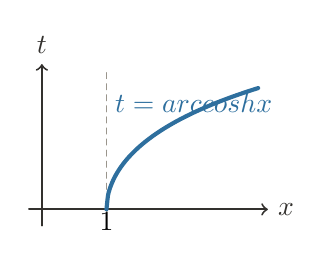
\begin{tikzpicture}[scale=0.82, line cap=round, line join=round]
  \draw[atlas axes] (-0.2,0)--(3.5,0) node[right] {$x$};
  \draw[atlas axes] (0,-0.25)--(0,2.25) node[above] {$t$};
  \draw[dropline] (1,-0.2)--(1,2.2);
  \glowstroke{atlasblue}{1:3.35}{ln(\x+sqrt(\x*\x-1))}
  \fill[atlas dot] (1,0) node[below] {$1$};
  \node[atlasblue] at (2.35,1.65) {$t=\operatorname{arccosh}x$};
\end{tikzpicture}

\atlascaption{HI2}{Inverse hyperbolic cosine}{Domain $[1,\infty)$ and range $[0,\infty)$; the inverse uses the nonnegative branch.}
\end{center}


\begin{definitionbox}{Definition}
\begin{definition}[Inverse hyperbolic cosine]
\label{def:inverse-hyperbolic-cosine}
The \emph{inverse hyperbolic cosine} function is the inverse of $\cosh$
after $\cosh$ is restricted to the interval $[0,\infty)$. It is denoted by
$\operatorname{arcosh}$ and has domain $[1,\infty)$ and range $[0,\infty)$.
\[
  \operatorname{arcosh} x=t
  \quad\Longleftrightarrow\quad
  \cosh t=x
  \quad\text{and}\quad
  t\geq 0.
\]
\end{definition}
\end{definitionbox}
\begin{remark*}[Standard quantified statement]
For every admissible input satisfying the hypotheses of the statement, the
displayed definition or assertion holds in the stated domain.
\end{remark*}

\begin{remark*}[Interpretation]
The statement records the named trigonometric object or identity together with
its intended domain of use.
\end{remark*}

\begin{remark*}[Domain and range]
The regular function $\cosh:\mathbb{R}\to[1,\infty)$ is even, so it is not
one-to-one on all of $\mathbb{R}$. The principal inverse uses the
nonnegative branch, where $\cosh$ increases from $1$ to infinity.
\end{remark*}
\begin{dependencies}
\begin{itemize}
  \item \hyperref[def:hyperbolic-cosine]{Hyperbolic cosine}
  \item \hyperref[thm:hyperbolic-sector-existence]{Existence for hyperbolic sectors}
  \item \hyperref[thm:hyperbolic-sector-uniqueness]{Uniqueness for hyperbolic sectors}
\end{itemize}
\end{dependencies}

\begin{theorembox}{Theorem}
\begin{theorem}[Principal inverse hyperbolic cosine identities]
\label{thm:inverse-hyperbolic-cosine-identities}
For every $x\in[1,\infty)$,
\[
  \cosh(\operatorname{arcosh} x)=x.
\]
For every $t\in[0,\infty)$,
\[
  \operatorname{arcosh}(\cosh t)=t.
\]
\end{theorem}
\end{theorembox}
\begin{remark*}[Standard quantified statement]
For every admissible input satisfying the hypotheses of the statement, the
displayed definition or assertion holds in the stated domain.
\end{remark*}

\begin{remark*}[Interpretation]
The statement records the named trigonometric object or identity together with
its intended domain of use.
\end{remark*}

\begin{remark*}[Proof]
These are the cancellation laws for the inverse of the restricted function
$\cosh|_{[0,\infty)}:[0,\infty)\to[1,\infty)$.
\end{remark*}
\begin{dependencies}
\begin{itemize}
  \item \hyperref[def:inverse-hyperbolic-cosine]{Inverse hyperbolic cosine}
\end{itemize}
\end{dependencies}
